\documentclass[../main.tex]{subfiles}
\begin{document}
\begin{itemize}
    \item \textbf{grandezze scalari:} $t,T,d,m,f,E,A.V,...$
    \item \textbf{grandezze vettoriali:} $\vec{v}, \vec{a}, \vec{F}, ...$
\end{itemize}

\vspace{1cm}
\begin{center}
    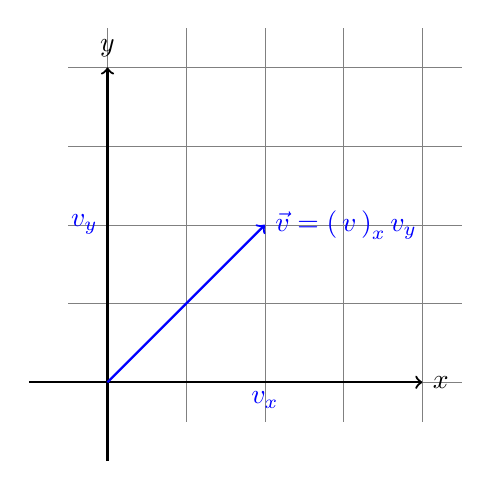
\begin{tikzpicture}
        % Disegna la griglia
        \draw[very thin, gray] (-0.5,-0.5) grid (4.5,4.5);
        
        % Disegna assi
        \draw[thick,->] (-1,0) -- (4,0) node[right] {$x$}; % Asse x
        \draw[thick,->] (0,-1) -- (0,4) node[above] {$y$}; % Asse y

        % Disegna la funzione y = 3x - 2
        \draw[->, domain=-0:2,smooth,variable=\x,blue,thick] 
        plot ({\x},{\x}) node[right] {$\vec{v}=\begin{pmatrix}
            v_x \\
            v_y
        \end{pmatrix}$};

        \node [blue,below] at (2, 0) {$v_x$};
        \node [blue,left] at (0, 2) {$v_y$};
    \end{tikzpicture}
\end{center}

\begin{align*}
    \left\lVert \vec{v}\right\rVert = v =& \sqrt{v_x^2 + v_y^2} \\
    v_x =& v \cdot cos(\alpha) \\
    v_y =& v \cdot sin(\alpha) \\
    v_y =& v_x \cdot tan(\alpha) \\
\end{align*}

Esiste una notazione alternativa, ecco alcuni esempi:
\begin{align*}
    \vec{v} =& \begin{pmatrix}
        3 \\
        6
    \end{pmatrix}
    = 3\hat{x} + 6\hat{y} \text{, $\hat{x}$ e $\hat{y}$ rappresentano dei versori} \\
    \vec{g} =& \begin{pmatrix}
        0 \\
        -9.81
    \end{pmatrix} \frac{m}{s^2}
    =(0\hat{x} - 9.81\hat{y}) \frac{m}{s^2}
\end{align*}

Proprietà utili:
\begin{itemize}
    \item Scomposizione
    \item Somma
    \item Prodotto tra un vettore e uno scalare
\end{itemize}

\pagebreak
\subsection{Vettori posizione, velocità, accellerazione e spostamento}
\begin{itemize}
    \item \textbf{vettori posizione:} $\vec{r}_a, \vec{r}_b$, $[m]$
    \item \textbf{vettore spostametno:} $\Delta\vec{r} = \vec{r}_b - \vec{r}_a$, $[m]$
\end{itemize}
\begin{center}
    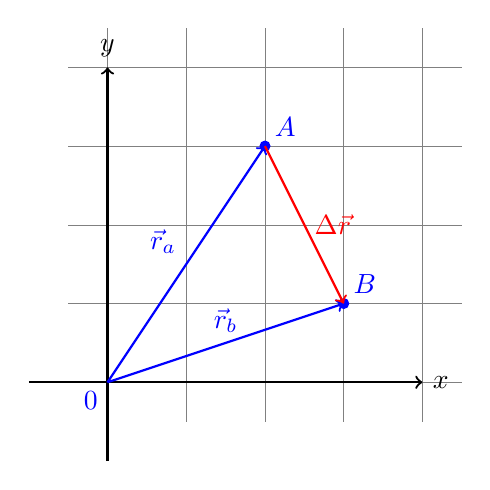
\begin{tikzpicture}
        % Disegna la griglia
        \draw[very thin, gray] (-0.5,-0.5) grid (4.5,4.5);
        
        % Disegna assi
        \draw[thick,->] (-1,0) -- (4,0) node[right] {$x$}; % Asse x
        \draw[thick,->] (0,-1) -- (0,4) node[above] {$y$}; % Asse y

        \draw[->, thick, blue] (0,0) -- (2,3) node[midway, above left] {$\vec{r}_a$};
        \draw[->, thick, blue] (0,0) -- (3,1) node[midway, above] {$\vec{r}_b$};
        \fill[blue] (2,3) circle (2pt) node[above right] {$A$};
        \fill [blue] (3,1) circle (2pt) node[above right] {$B$};

        \draw[->, thick, red] (2,3) -- (3,1) node[midway, right] {$\Delta\vec{r}$};

        \node [blue,below left] at (0, 0) {$0$};
    \end{tikzpicture}
\end{center}

\vspace{1.25cm}
\begin{itemize}
    \item \textbf{velocità media:} $\vec{V}_m = \frac{\Delta\vec{ r}}{\Delta t}$
    \begin{itemize}
        \item $[\frac{m}{s}]$
        \item $\left\lVert \vec{V}_m\right\rVert = V_m = \frac{\Delta r}{\Delta t} $
        \item $\vec{V}_m\upuparrows \Delta\vec{r}$, equiverso (stessa direzione e stesso verso)
    \end{itemize}
    \item \textbf{Velocità istantanea:} $\vec{V}_{ist} = \lim\limits_{\Delta t \to 0}\vec{V}_m $, tangente alla traiettoria
\end{itemize}
\begin{center}
    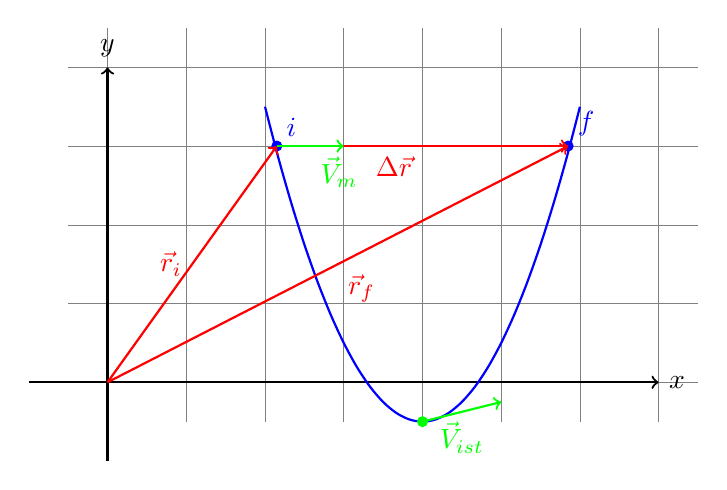
\begin{tikzpicture}
        % Disegna la griglia
        \draw[very thin, gray] (-0.5,-0.5) grid (7.5,4.5);
        
        % Disegna assi
        \draw[thick,->] (-1,0) -- (7,0) node[right] {$x$}; % Asse x
        \draw[thick,->] (0,-1) -- (0,4) node[above] {$y$}; % Asse y

        % Disegna la funzione y = 3x - 2
        \draw[domain=2:6,smooth,variable=\x,blue,thick] 
        plot (\x, {-2(\x-4)^2 -0.5}) node[above] {};


        \fill[blue] (2.15,3) circle (2pt) node[above right] {$i$};
        \fill [blue] (5.85,3) circle (2pt) node[above right] {$f$};

        \draw[->, thick, red] (0,0) -- (2.15,3) node[midway, left] {$\vec{r}_i$};
        \draw[->, thick, red] (0,0) -- (5.85,3) node[midway, below right] {$\vec{r}_f$};

        \draw[->, thick, red] (2.15,3) -- (5.85,3) node[midway, below left] {$\Delta\vec{r}$};
        \draw[->, thick, green] (2.15,3) -- (3,3) node[midway, below right] {$\vec{V}_m$};

        \fill [green] (4,-0.5) circle (2pt) node[above right] {};
        \draw[->, thick, green] (4,-0.5) -- (5,-0.25) node[midway, below ] {$\vec{V}_{ist}$};
    \end{tikzpicture}
\end{center}

\vspace{1.25cm}
\begin{itemize}
    \item \textbf{Accellerazione media:} $\vec{a}_m = \frac{\Delta \vec{V}_m}{\Delta t}$
    \begin{itemize}
        \item $[\frac{m}{s^2}]$
        \item $\left\lVert \vec{a}_m\right\rVert = a_m = \frac{\Delta V_m}{\Delta t} $
        \item $\vec{a}_m\upuparrows \Delta\vec{V}_m$, equiversi
        \begin{itemize}
            \item \textit{attenzione:} $\Delta \vec{V}_m = \vec{V}_f - \vec{V}_i$
        \end{itemize}
        \item \textbf{Accellerazione istantanea:} $\vec{a}_{ist} = \lim\limits_{\Delta t \to 0}\vec{a}_m $
    \end{itemize}
\end{itemize}
\textbf{Nota:} nel caso dell'accellerazione i vettori puntano verso il centro della circonferenza.

\end{document}